\section{Gr\"obner Bases}

The contents here contained are a summary of the information provided in class with Chapter 2, sections 1-8 of \textit{Ideals, Varieties, and Algorithms} by Cox \textit{et. al}.

\subsection{Introduction}

\begin{definition}[Polynomial]
    A \textit{polynomial} $f$ in $x_1, \dots, x_n$ with coefficients in a field $k$ is a finite linear combination (with coefficients in $k$) of monomials.
    The set of all polynomials in $x_1, \dots, x_n$ with coefficients in $k$ is denoted $k[x_1, \dots, x_n]$.
\end{definition}

\begin{definition}[Affine Space]
    Given a field $k$ and a positive integer $n$, we define the $n$-dimensional \textit{affine space} over $k$ to be the set
    $$k^n = \{ (a_1, \dots, a_n) | a_1, \dots, a_n \in k \}$$
\end{definition}

\begin{definition}[Affine Variety]
    Let $k$ be a field and let $f_1, \dots, f_s$ be polynomials in $k[x_1, \dots, x_n]$.
    Then the affine variety defined by $f_1, \dots, f_s$ is,
    $$\pmb{V}(f_1, \dots, f_s) = \{ (a_1, \dots, a_n) \in k^n | f_i(a_1, \dots, a_n) = 0 \quad \forall 1 \leq i \leq s \}$$
\end{definition}

\begin{definition}[Ideals]
    A subset $I \subseteq k[x_1, \dots, x_n]$ is an \textit{ideal} if it satisfies:
    \begin{enumerate}
        \item[(i)] $0 \in I$
        \item[(ii)] If $f, g \in I$, then $f + g \in I$
        \item[(iii)] If $f \in I$ and $h \in k[x_1, \dots, x_n]$ then $hf \in I$.
    \end{enumerate}
    Additionally, let $f_1, \dots, f_s$ be polynomials in $k[x_1, \dots, x_n]$.
    Then,
    $$\langle f_1, \dots, f_s\rangle = \left\{ \sum_{i=1}^s h_i f_i | h_1, \dots, h_s \in k[x_1, \dots, x_n] \right\}$$
    is the \textit{ideal generated} by $f_1, \dots, f_s$.

    Lastly, if $V \subseteq k^n$ is an affine variety, the set
    $$\pmb{I}(V) = \{f \in k[x_1, \dots, x_n] | f(a_1, \dots, a_n) = 0 \quad \forall (a_1, \dots, a_n) \in V\}$$
    is \textit{the ideal of V}.
\end{definition}

\subsection{Orderings on the Monomials}

\begin{definition}[Monomial Ordering]
    A \textit{monomial ordering} > on $k[x_1, \dots, x_n]$ is a relation $>$ on $\Z^n_{\geq 0}$, or equivalently, a relation on the set if monomials $x^{\alpha}$, $\alpha \in \Z^n_{\geq 0}$, satisfying:
    \begin{enumerate}
        \item[(i)] $>$ is a total (or linear) ordering on $\Z^n_{\geq 0}$
        \item[(ii)] If $\alpha > \beta$ and $\gamma \in \Z^n_{\geq 0}$, then $\alpha + \gamma > \beta + \gamma$.
        \item[(iii)] $>$ is a well-ordering on $\Z^n_{\geq 0}$.
            This means that every nonempty subset of $\Z^n_{\geq 0}$ has a smallest element under $>$.
    \end{enumerate}
\end{definition}

\begin{definition}[Lexicographical Order]
    Let $\alpha = (\alpha_1, \dots, \alpha_n)$ and $\beta = (\beta_1, \dots, \beta_n)$ be in $\Z^n_{\geq 0}$.
    We say $\alpha >_{lex} \beta$ if the leftmost nonzero entry of the vector difference $\alpha - \beta \in \Z^n$ is positive.
    We will write $x^{\alpha} >_{lex} x^{\beta}$ if $\alpha >_{lex} \beta$.
\end{definition}

\begin{definition}[Graded Lex Order]
    Let $\alpha, \beta \in \Z^n_{\geq 0}$.
    We say $\alpha >_{grlex} \beta$ if
    $$|\alpha| = \sum_{i=1}^n \alpha_i > |\beta| = \sum_{i=1}^n \beta_i, \quad or \quad |\alpha | = | \beta | \text{ and } \alpha >_{lex} \beta$$
\end{definition}

\begin{definition}[Graded Reverse Lex Order]
    Let $\alpha, \beta \in \Z^n_{\geq 0}$.
    We say $\alpha >_{grlex} \beta$ if
    $$|\alpha| = \sum_{i=1}^n \alpha_i > |\beta| = \sum_{i=1}^n \beta_i, \quad or \quad |\alpha | = | \beta | \text{ and the rightmost nonzero entry of } \alpha - \beta \text{ is negative }$$
\end{definition}

\begin{theorem}[Division Algorithm]
    Let $>$ be a monomial order on $\Z^n_{\geq 0}$ and let $F = (f_1, \dots, f_s)$ be an ordered $s$-tuple of polynomials in $k[x_1, \dots, x_n]$.
    Then, every $f \in k[x_1, \dots, x_n]$ can be written as:
    $$f = q_1f_1 + \dots + q_sf_s + r$$
    where $q_i, r \in k[x_1, \dots, x_n]$, and either $r = 0$ or it is a linear combination, with coefficients in $k$, of monomials none of which is divisible by any of $LT(f_1), \dots, LT(f_s)$.
    The algorithm is depicted in Figure~\ref{fig:division-algorithm}.
\end{theorem}
\begin{figure}[h!]
    \centering
    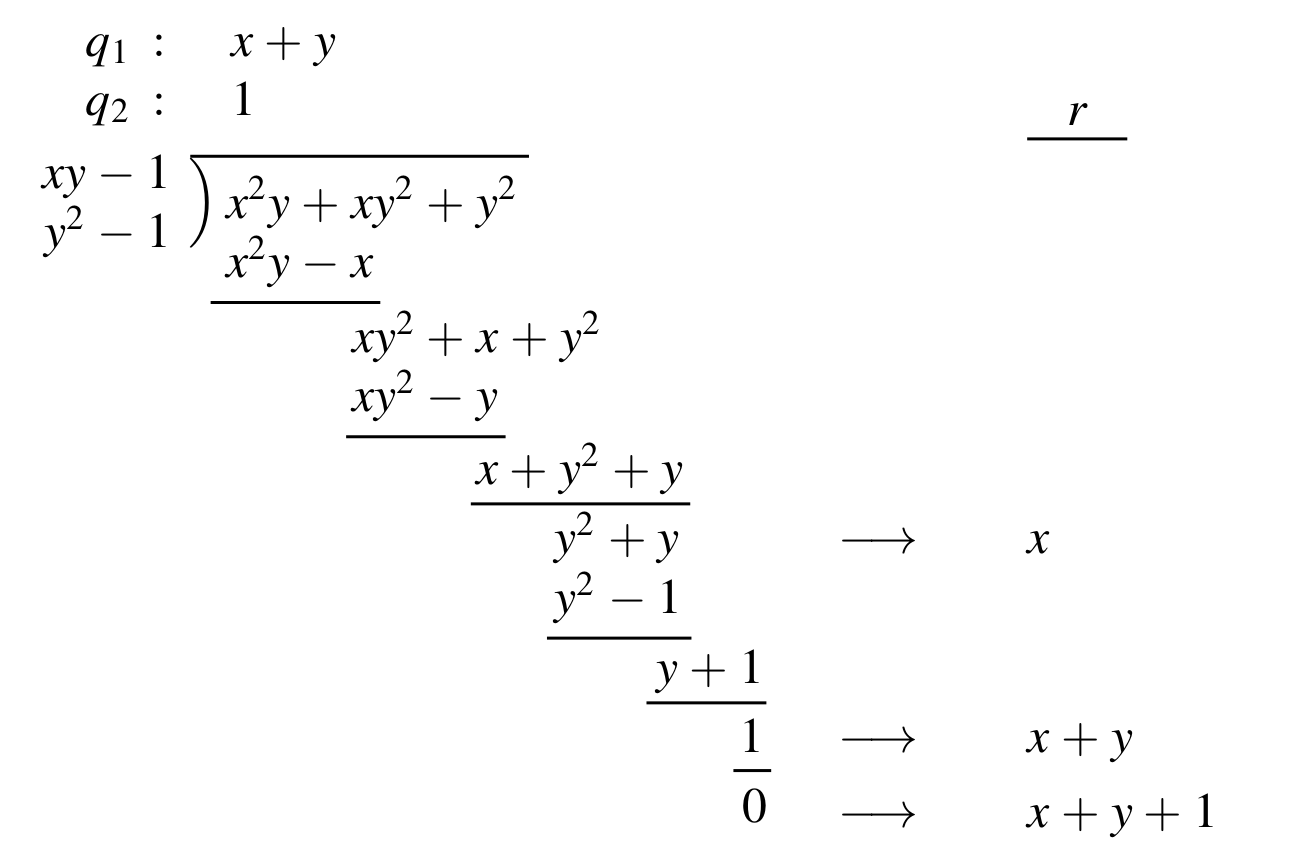
\includegraphics[width=.6\textwidth]{img/division.png}
    \caption{Division algorithm for polynomials.\label{fig:division-algorithm}}
\end{figure}

Note that, with the defined division algorithm, we can check for ideal membership by dividing by all the ideal generators and checking the remainder (sufficient, but not necessary). I.e. depending on the order we give to $(f_1, \dots, f_s)$ the remainder may vary.
Gr\"obner bases will solve this problems.

\subsection{Monomial Ideals}

\begin{definition}[Monomial Ideal]
    An ideal $I \subseteq k[x_1, \dots, x_n]$ is a \textit{monomial ideal} if there is a subset $A \subseteq \Z^n_{\geq 0}$ (possibly infinite) such that $I$ consists of all polynomials which are finite sums of the form $\sum_{\alpha \in A} h_{\alpha}x^{\alpha}$, where $h_{\alpha} \in k[x_1, \dots, x_n]$. In this case, we write $I = \langle x^{\alpha} | \alpha \in A \rangle$.
\end{definition}

\begin{lemma}
    Let $I = \langle x^{\alpha} | \alpha \in A \rangle$ be a monomial ideal.
    Then a monomial $x^{\beta}$ lies in $I$ if and only if $x^{\beta}$ is divisible by $x^{\alpha}$ for some $\alpha \in A$.
\end{lemma}

\begin{lemma}
    Let $I$ be a monomial ideal, and let $f \in k[x_1, \dots, x_n]$.
    Then the following are equivalent:
    \begin{enumerate}
        \item[(i)] $f \in I$.
        \item[(ii)] Every term of $f$ lies in $I$.
        \item[(iii)] $f$ is a $k$-linear combination of the monomials in $I$.
    \end{enumerate}
\end{lemma}

\begin{lemma}[Dickson's Lemma]
    Let $I = \langle x^{\alpha} | \alpha \in A \rangle \subseteq k[x_1, \dots, x_n]$ be a monomial ideal.
    Then I can be written in the form $I = \langle x^{\alpha(1)}, \dots, x^{\alpha(s)} \rangle$, where $\alpha(1), \dots, \alpha(s) \in A$. In particular, $I$ has a finite basis.
\end{lemma}

\subsection{The Hilbert Basis Theorem and Gr\"obner Bases}

\begin{definition}[Ideal of Leading Terms]
    Let $I \subseteq k[x_1, \dots, x_n]$ be an ideal, and fix a monomial ordering on $k[x_1, \dots, x_n]$.
    Then:
    \begin{enumerate}
        \item[(i)] We denote by $LT(I)$ the set of leading terms of nonzero elements of $I$.
        \item[(ii)] We denote by $\langle LT(I) \rangle$ the ideal generated by the elements of $LT(I)$.
    \end{enumerate}
\end{definition}

\begin{lemma}
    Let $ I \subseteq k[x_1, \dots, x_n]$ be an ideal different from $\{ 0 \}$.
    \begin{enumerate}
        \item[(i)] $\langle LT(I) \rangle$ is a monomial ideal.
        \item[(ii)] There are $g_1, \dots, g_t \in I$ such that $\langle LT(I) \rangle = \langle LT(g_1), \dots, LT(g_t) \rangle$.
    \end{enumerate}
\end{lemma}

\begin{theorem}[Hilbert Basis Theorem]
    Every polynomial ideal $I \subseteq k[x_1, \dots, x_n]$ has a finite generating set.
    In other words, $I = \langle g_1, \dots, g_t \rangle$ for some $g_1, \dots, g_t \in I$.
\end{theorem}

\begin{definition}[Gr\"obner (or Standard) Basis]
    Fix a monomial order on the polynomial ring $k[x_1, \dots, x_n]$.
    A finite subset $G = \{g_1, \dots, g_t \}$ of an ideal $I \subseteq k[x_1, \dots, x_n]$ different from $\{ 0 \}$ is said to be a \textit{Gr\"obner (or Standard) Basis} if
    $$ \langle LT(g_1), \dots, LT(g_t) \rangle = \langle LT(I) \rangle$$
    Equivalently, $G$ is a Gr\"obner Basis of $I$ if and only if the leading term of any element of $I$ is divisible by one of the $LT(g_i)$.
\end{definition}

\begin{proposition}
    Let $G = \{ g_1, \dots, g_t \}$ be a Gr\"obner basis for an ideal $I \subseteq k[x_1, \dots, x_n]$ and let $f \in k[x_1, \dots, x_n]$.
    Then, $f \in I$ if and only if the remainder on division of $f$ by $G$ is zero (no matter how the elements of $G$ are listed when using the division algorithm).
\end{proposition}

\begin{definition}[LCM and S-Polynomial]
    Let $f, g \in k[x_1, \dots, x_n]$ be nonzero polynomials.
    \begin{enumerate}
        \item[(i)] If multideg$(f) = \alpha$ and multideg$(g) = \beta$, then let $\gamma = (\gamma_1, \dots, \gamma_n)$, where $\gamma_i = \max(\alpha_i, \beta_i)$ for each $i$.
            Then, $x^{\gamma}$ is the \textit{least common multiple} of $LM(f)$ and $LM(g)$ (leading monomials).
        \item[(ii)] The \textit{S-Polynomial} of $f$ and $g$ is the combination
            $$S(f,g) = \frac{x^{\gamma}}{LT(f)} \cdot f - \frac{x^{\gamma}}{LT(g)} \cdot g$$
    \end{enumerate}
\end{definition}

\begin{theorem}[Buchberger's Criterion]
    Let $I$ be a polynomial ideal.
    Then a basis $G = \{ g_1, \dots, g_t \}$ of $I$ is a Gr\"obner basis of $I$ if and only if for all pairs $i \neq j$, the remainder on division of $S(g_i, g_j)$ by $G$ (listed in some order) is zero.
\end{theorem}

\begin{theorem}[Buchberger's Algorithm]
    Let $I = \langle f_1, \dots, f_s \rangle \neq \{ 0 \}$ be a polynomial ideal.
    Then a Gr\"obner basis for $I$ can be constructed in a finite number of steps by the following algorithm:
\end{theorem}
\begin{figure}[h!]
    \centering
    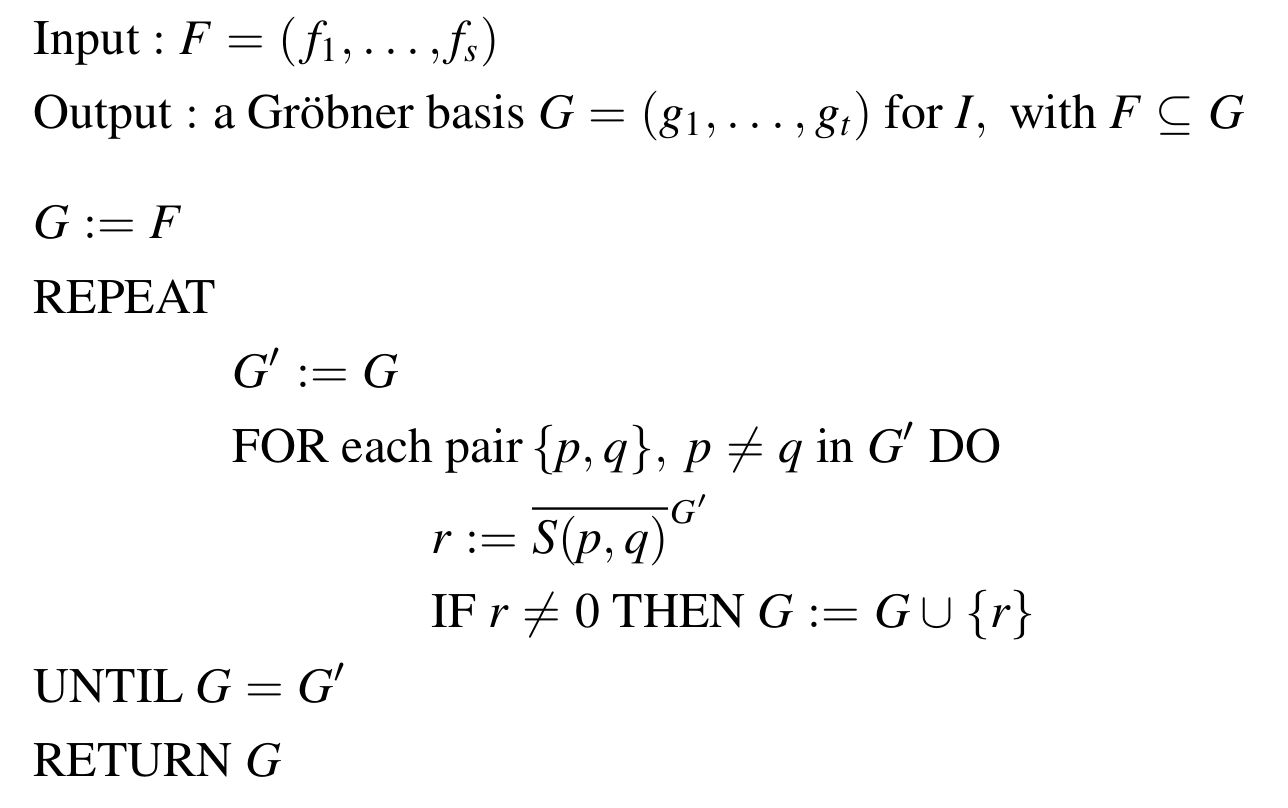
\includegraphics[width=.5\textwidth]{img/grobner_algo.png}
\end{figure}

\begin{definition}[Reduced Gr\"obner Basis]
    A \textit{reduced Gr\"obner basis} for a polynomial ideal $I$ is a Gr\"obner basis $G$ for $I$ such that:
    \begin{enumerate}
        \item[(i)] $LC(p) = 1$ for all $p \in G$.
        \item[(ii)] For all $p \in G$, no monomial of $p$ lies in $\langle LT(G \backslash \{ p \}) \rangle$.
    \end{enumerate}
    Further, given a monomial ordering, the reduced Gr\"obner basis is unique.
\end{definition}

\subsection{The Elimination Theorem}

\begin{definition}[$l$-th Elimination Ideal]
    Given $I = \langle f_1, \dots, f_s \rangle \subseteq k[x_1, \dots, x_n]$, the \textit{$l$-th elimination ideal $I_l$} is the ideal of $k[x_{l+1}, \dots, x_n]$ defined by,
    $$I_l = I \cap k[x_{l+1}, \dots, x_n]$$
\end{definition}

\begin{theorem}[The Elimination Theorem]
    Let $I \subseteq k[x_1, \dots, x_n]$ be an ideal and let $G$ be a Gr\"obner basis of $I$ with respect to lex order where $x_1 > x_2 > \dots > x_n$.
    Then, for every $0 \leq l \leq n$, the set
    $$G_l = G \cap k[x_{l+1}, \dots, x_n]$$
    is a Gr\"obner basis of the $l$-th elimination ideal $I_l$.
\end{theorem}
